%%%%%%%%%%%%%%%%%%%%%%%%%%%%%%%%%%%%%%%%%%%%%%%%%%%%%%%%%%%%%%%%%%%%%%%%%%%
% Chapter 3: Confidence intervals and hypothesis testing
%%%%%%%%%%%%%%%%%%%%%%%%%%%%%%%%%%%%%%%%%%%%%%%%%%%%%%%%%%%%%%%%%%%%%%%%%%%

\Chapter{Chapter 3}{Confidence intervals and hypothesis testing}{Chapter 3: Confidence intervals and hypothesis testing}
{
Please read Section 7.2, Chapter 9, Chapter 10, Section 11.1 - 11.7, Section 13.9, Section 14.7, and Section 14.9 from \textit{\href{https://learningstatisticswithr.com/}{{\color{black}Learning Statistics with R}}} before starting these assignments.
}

\fancyhead[R]{\fontsize{12}{14}\selectfont\textit{Chapter 3: Confidence intervals and hypothesis testing}}

\chaptertitle{Chapter 3: Confidence intervals and hypothesis testing}

\learningobjectives{
    \item Confidence interval and hypothesis testing by hand
    \item Testing the homogeneity of variance by hand
    \item Calculating confidence intervals for the mean and testing for normality
    \item Inspect and test the normality of a sample in R
    \item Using R to inspect and test the homogeneity of variance
}

% To add an assignment to the chapter, create a file in the folder "Assignments" and insert the link below

%%%%%%%%%%%%%%%%%%%%%%%%%%%%%%%%%%%%%%%%%%%%%%%%%%%%%%%%%%%%%%%%%%%%%%%%%%%
% Assignment 3.1: Confidence interval and hypothesis testing by hand
%%%%%%%%%%%%%%%%%%%%%%%%%%%%%%%%%%%%%%%%%%%%%%%%%%%%%%%%%%%%%%%%%%%%%%%%%%%

\handassignment{Assignment 3.1: Confidence interval and hypothesis testing by hand}

A call center with 38 employees handles thousands of calls a day. The company wants to get more insights into the duration of calls and the workload of the employees. On a day with a total of 4513 calls, the company decides to randomly pick 100 calls and measure how long they take. The \concept{mean} call duration for this sample is 145 seconds with a \concept{standard deviation} of 25 seconds. The call center wants to use this information to estimate the \concept{mean} call duration for that day. \\

\question{
    3.1 a
}{
    Write down the relevant information from this case. Use the symbols $N$, $n$, $\bar{x}$, $s$, $\sigma$, and $\mu$.
}

\hint{Hint 3.1: Not all symbols are known and some should be left empty.}

\emptyanswerbox{
    3.1a
}{
        $N$: \shortanswerline \hspace{1cm} \quad $s$: \shortanswerline
            \answerbreak
            $n$: \shortanswerline \hspace{1cm} \quad $\sigma$: \shortanswerline
            \answerbreak
            $\bar{x}$: \shortanswerline \hspace{1cm} \quad $\mu$: \shortanswerline
}

\question{
    3.1 b
}{
    What is the best estimate of the \concept{mean} call duration ($\mu$) based on this sample?
}

\emptyanswerbox{
    3.1b
}{
    $\mu = $\shortanswerline    
    \answerskip
    Explanation:
    \answerskip
    \rule{\textwidth}{0.4pt}
}

\clearpage % Page break

\question{
    3.1 c
}{
    Calculate the \concept{standard error} of the mean ($SE_\mu$) based on this sample.
}

\hint{Hint 3.2: Check the formula sheet to find out how to calculate $SE_\mu$.}

\emptyanswerbox{
    3.1c
}{
    $SE_\mu = $\shortanswerline    
    \answerskip
    Calculation:
    \answerskip
    \rule{\textwidth}{0.4pt}
}

\question{
    3.1 d
}{
    Calculate the 99\% \concept{confidence interval} for the mean call duration.
}

\hint{Hint 3.3: You can find the formula for the \concept{lower bound}, \concept{upper bound} and \concept{z-value} in the formula sheet.}

\emptyanswerbox{
    3.1d
}{
    z-value: \qquad \shortanswerline    
    \answerskip
    Calculation: \mediumanswerline
    \answerskip
    \answerskip
    Lower bound: \shortanswerline    
    \answerskip
    Calculation: \mediumanswerline
    \answerskip
    \answerskip
    Upper bound: \shortanswerline    
    \answerskip
    Calculation: \mediumanswerline
    \answerskip
}

The manager of the call center does not really care about the \concept{lower bound} and he does not require such high confidence. He just wants to make sure the average workload per employee is not too high, because otherwise he is forced by employment laws to hire more people. He calculated that if the \concept{mean} call duration is below 150 seconds the workload is acceptable, and wants to use this sample to show with 95\% confidence that the \concept{mean} call duration is below 150 seconds. \\

\clearpage % Page break

\question{
    3.1 e
}{
    Write down the hypotheses $H_0$ and $H_1$ for the manager’s test. What is the value of $\mu_0$? Also describe $\mu_0$ for this case. 
}

\hint{Hint 3.4: This is a one-sided test. Consider this when you formulate the hypotheses.}

\emptyanswerbox{
    3.1e
}{
    $\mu_0$: \shortanswerline    
    \answerskip
    $H_0$: \shortanswerline \hspace{5cm} $H_1$: \shortanswerline
}

\question{
    3.1 f
}{
    Do you need the \concept{lower bound} or the \concept{upper bound} of the \concept{confidence interval} for this test? Calculate this bound. 
}

\emptyanswerbox{
    3.1f
}{
    ........ bound: \shortanswerline    
    \answerskip
    Calculation: \qquad \hspace*{5pt} \mediumanswerline
}

\question{
    3.1 g
}{
    Draw the conclusion for the manager. Include the following four elements:
    \begin{itemize}
        \item[$\square$] Show how the \concept{confidence interval} relates to $\mu_0$.
        \item[$\square$] Discuss whether $H_0$ is rejected or not.
        \item[$\square$] Describe what this tells us about $\mu$ and $\mu_0$.
        \item[$\square$] Describe what type of error is relevant \textit{(type-I or type-II)}.
    \end{itemize}
}

\sixlineanswerbox{3.1g}

\clearpage % Page break
%%%%%%%%%%%%%%%%%%%%%%%%%%%%%%%%%%%%%%%%%%%%%%%%%%%%%%%%%%%%%%%%%%%%%%%%%%%
% Assignment 3.2: Testing for homogeneity of variance by hand
%%%%%%%%%%%%%%%%%%%%%%%%%%%%%%%%%%%%%%%%%%%%%%%%%%%%%%%%%%%%%%%%%%%%%%%%%%%

\handassignment{Assignment 3.2: Testing for homogeneity of variance by hand}

A manufacturer of machines for food processing has created a machine that fills bags with sugar. A machine like this is never perfect and when a 1-kilo bag of sugar is filled there are always small deviations. the actual content of a bag is often a few grams more or less than a kilo. The manufacturer knows these deviations are bigger for new machines but become smaller as the machine is longer used due to better calibration and the smoothing out of the moving parts. To be able to show this to his clients they take a random sample of eight bags of sugar on the first day of the three months the machine is in use and plots the (absolute) weight deviations. \\

The manufacturer wants to use the chart below for a model that shows how much the machine improves over time, but this requires \concept{homogeneity of variances}. The \concept{variance} in month 1 is 0.801 gr, the \concept{variance} in month 2 is 1.113 gr. The \concept{variance} for month 3 has not been calculated yet. \\

\begin{minipage}[t]{0.5\textwidth}
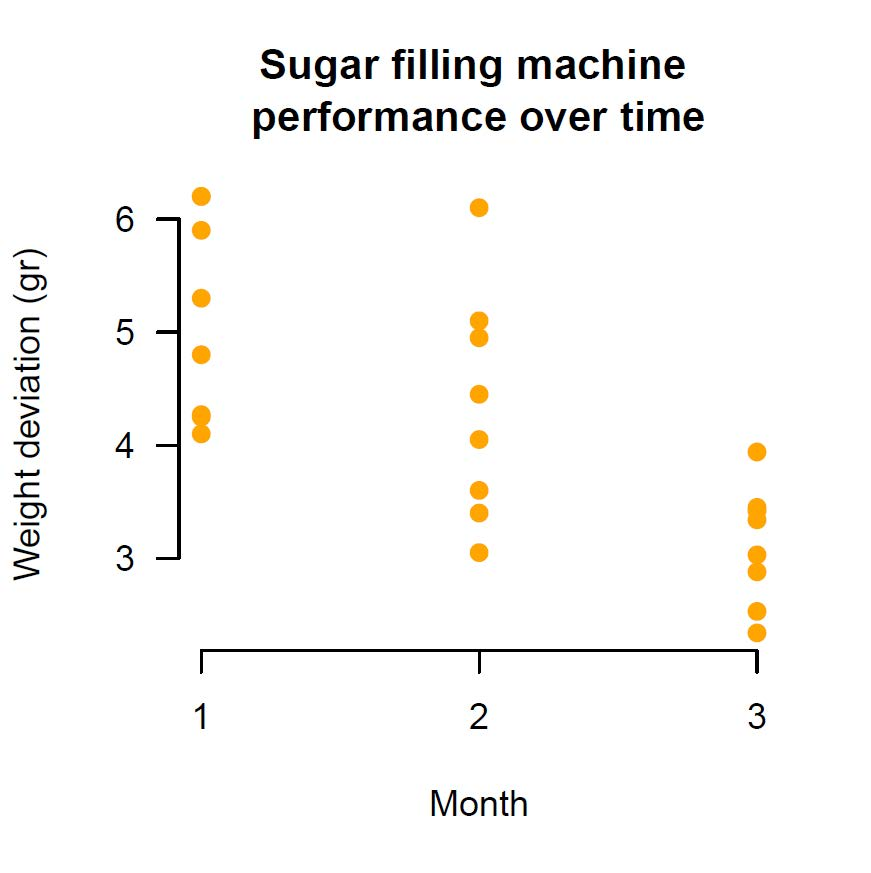
\includegraphics[width=\textwidth]{Files/Images/homogeneityOfVariances.jpg}
\end{minipage}%
\begin{minipage}[t]{0.5\textwidth}
\vspace*{-7cm}
\begin{center}
    \begin{tabular}{|c|c|c|c|}
    \hline 
    $i$ & $x_i$ & $(x_i - \bar{x})$ & $(x_i - \bar{x})^2$ \tstrut\bstrut\\
    \hline
    1 & 3.03 & & \tstrut\bstrut\\
    \hline
    2 & 3.45 & & \tstrut\bstrut\\
    \hline
    3 & 3.94 & & \tstrut\bstrut\\
    \hline
    4 & 2.34 & & \tstrut\bstrut\\
    \hline
    5 & 3.34 & & \tstrut\bstrut\\
    \hline
    6 & 2.53 & & \tstrut\bstrut\\
    \hline
    7 & 2.88 & & \tstrut\bstrut\\
    \hline
    8 & 3.42 & & \tstrut\bstrut\\
    \hline
    \end{tabular}
    \end{center}
    
    $\sum x_i = $  ............. \hspace*{.4cm} $\sum (x_i - \bar{x})^2 = $  ............. \\
    \\
    \hspace*{10pt} $\bar{x} = $ ............. \hspace*{2cm} $s^2 = $  ............. \\
\end{minipage}%

\question{
    3.2 a
}{
    Use the table to the right of the figure to calculate the \concept{variance} $s^2$ for month 3 by filling in the calculations beneath the table.
}

\hint{Hint 3.5: you can find the formula for the \concept{variance} in the formula sheet.}

\emptyanswerbox{
    3.2a
}{
    Variance: \shortanswerline
}   

\question{
    3.2 b
}{
    Calculate \concept{Hartley’s F} (the variance ratio) for the sugar machine data set.
}

\hint{Hint 3.6: you can find the formula for \concept{Hartley’s F} in the formula sheet.}

\clearpage % Page break

\emptyanswerbox{
    3.2b
}{
    Hartley's F: \shortanswerline
}   

\question{
    3.2 c
}{
    Formulate the \concept{null hypothesis} $H_0$ and \concept{alternative hypothesis} $H_1$ to test homogeneity of variance for this case.
}

\hypothesesbox{3.2c}

\question{
    3.2 d
}{
    Determine the \concept{critical value} for Hartley’s F ($F_{\max}$) for the sugar machine data set.
}

\hint{Hint 3.7: Check Table 1 in the formula sheet for the critical values of \concept{Hartley’s F}.}

\emptyanswerbox{
    3.2d
}{
    Hartley's $F_{\max}$: \shortanswerline
}   

\question{
    3.2 e
}{
    Draw the conclusion on the homogeneity of variance for the sugar machine data set. Include the following elements:
    \begin{itemize}
        \item[$\square$] Show how the calculated \concept{Hartley's F} relates to the critical value $F_{max}$.
        \item[$\square$] Discuss whether $H_0$ is rejected or not.
        \item[$\square$] Describe what this tells us about the homogeneity of the three variances.
        \item[$\square$] Describe what type of error is relevant \textit{(type-I or type-II)}.
    \end{itemize}
}

\sixlineanswerbox{3.2e}

\clearpage % Page break
%%%%%%%%%%%%%%%%%%%%%%%%%%%%%%%%%%%%%%%%%%%%%%%%%%%%%%%%%%%%%%%%%%%%%%%%%%%
% Assignment 3.3: Calculating the confidence interval for the mean and
% testing for normality
%%%%%%%%%%%%%%%%%%%%%%%%%%%%%%%%%%%%%%%%%%%%%%%%%%%%%%%%%%%%%%%%%%%%%%%%%%%

\rassignment{Assignment 3.3: Calculating a confidence interval and
testing for normality}

For this assignment, you will need the \dataset{populations.csv} data file, which contains four different \concept{populations} of 10,000 observations called \rcode{P1 - P4}. \\

\question{
    3.3 a
}{
    Use the \rcode{read.csv()} function (and \rcode{setwd()} function if you prefer) to import the data set into an object named \rcode{dataset5}.
}

\rcodeanswertiny{3.3a}

\question{
    3.3 b
}{
    Run the following code in \texttt{R} and explain what it does. Why do you have to use a seed?
}

\codeblock{set.seed(54321) {\color{dataset} \# You can replace 54321 with your own seed number} \\
\\
sample1 <- sample(dataset5\$P1, size = 90)\\
sample2 <- sample(dataset5\$P2, size = 90)\\
sample3 <- sample(dataset5\$P3, size = 90)\\
sample4 <- sample(dataset5\$P4, size = 90)
}

\hint{Hint 3.8: Use R’s help function \rcode{?} to look for the \rcode{sample()} and \rcode{set.seed()} functions.}

\twolineanswerbox{3.3b}

\question{
    3.3 c
}{
    Calculate the \concept{mean} and \concept{standard deviation} for each \concept{sample} and save them into variables \rcode{x1} - \rcode{x4} and \rcode{s1} - \rcode{s4}. Use these results to also calculate the \concept{standard errors} and same them into variables \rcode{se1} - \rcode{se4}.
}

\rcodeanswermedium{3.3c}

\clearpage % Page break

\emptyanswerbox{
    3.3c
}{
    Standard error sample 1: \shortanswerline
    \answerskip
    Standard error sample 2: \shortanswerline
    \answerskip
    Standard error sample 3: \shortanswerline
    \answerskip
    Standard error sample 4: \shortanswerline
}

The \texttt{R} function \rcode{qnorm(p, mean, sd)} returns the \concept{z-value} for \concept{quantile} \rcode{p} from a \concept{normal distribution} with a certain \concept{mean} $\mu$ (\rcode{mean}) and \concept{standard deviation} $\sigma$ (\rcode{sd}). If you do not specify a mean or standard deviation for the function it will assume the standard normal distribution $N(\mu = 0, \sigma = 1)$. \\

\question{
    3.3 d
}{
    Run the following code in \texttt{R} and explain the value that you see. 
}

\codeblock{qnorm(p = 0.95)}

\twolineanswerbox{3.3d}

The \rcode{qnorm()} function cannot return the \concept{z-value} for the two-sided \concept{confidence interval}, but you can work around that by realizing that in a two-sided interval you have to split the risk over both sides of the standard normal distribution. \\

\question{
    3.3 e
}{
    Run the following code in \texttt{R} and explain why you can use the value in \rcode{z} for a two-sided 95\% \concept{confidence interval}. 
}

\codeblock{z <- qnorm(p = 0.975)}

\twolineanswerbox{3.3e}

\question{
    3.3 f
}{
    Calculate the 95\% \concept{confidence interval} for each sample. Store the lower bounds \rcode{lb1} - \rcode{lb4} and store the upper bounds in \rcode{ub1} - \rcode{ub4}.
}

\clearpage % Page break

\rcodeanswermedium{3.3f}

This is a rare case in which you actually have the full \concept{populations}, so you can check if the estimates based on your \concept{samples} are actually close to the real value in the populations. \\

\question{
    3.3 g
}{
    Calculate the actual \concept{population means}, call them \rcode{mu1} - \rcode{mu4}. Next, fill the schema below with all known values for \rcode{ub}, \rcode{x}, \rcode{lb}, and \rcode{mu}. 
}

\rcodeanswermedium{3.3g}

\emptyanswerbox{
    3.3g
}{
    \vspace*{-10pt}
    \begin{center}
    \begin{tabular}{r|c|c|c|c|}
    \multicolumn{1}{c}{} & \multicolumn{1}{c}{\rcode{sample1}} & \multicolumn{1}{c}{\rcode{sample2}} & \multicolumn{1}{c}{\rcode{sample3}} & \multicolumn{1}{c}{\rcode{sample4}} \tstrut\bstrut\\
    \cline{2-5}
    \rcode{ub} & & & & \tstrut\bstrut\\
    \cline{2-5}
    \rcode{x} & & & & \tstrut\bstrut\\
    \cline{2-5}
    \rcode{lb} & & & & \tstrut\bstrut\\
    \cline{2-5}
    \end{tabular}
    \end{center}
    
    \begin{center}
    \begin{tabular}{r|c|c|c|c|}
    \multicolumn{1}{c}{} & \multicolumn{1}{c}{\rcode{P1}} & \multicolumn{1}{c}{\rcode{P2}} & \multicolumn{1}{c}{\rcode{P3}} & \multicolumn{1}{c}{\rcode{P4}} \tstrut\bstrut\\
    \cline{2-5}
    \rcode{mu} & & & & \tstrut\bstrut\\
    \cline{2-5}
    \textit{mu in interval?} & YES / NO & YES / NO & YES / NO & YES / NO \tstrut\bstrut\\
    \cline{2-5}
    \end{tabular}
    \end{center}
}

\question{
    3.3 h
}{
    Are all \concept{population means} inside the interval you calculated?
}

\emptyanswerbox{
    3.3h
}{
    \vspace*{-15pt}
    \begin{center}
        YES / NO
    \end{center}
}

\question{
    3.3 i
}{
    How often do you expect this to happen given the confidence level (95\%) used?
}

\onelineanswerbox{3.3i}

\clearpage % Page break
%%%%%%%%%%%%%%%%%%%%%%%%%%%%%%%%%%%%%%%%%%%%%%%%%%%%%%%%%%%%%%%%%%%%%%%%%%%
% Assignment 3.4: Inspect and test the normality of a sample in R
%%%%%%%%%%%%%%%%%%%%%%%%%%%%%%%%%%%%%%%%%%%%%%%%%%%%%%%%%%%%%%%%%%%%%%%%%%%

\rassignment{Assignment 3.4: Inspecting and testing the normality of a sample in R}

In this assignment you are going to work with an \texttt{R} package called \rcode{car}. Packages are extensions for \texttt{R} created by its community. They contain functions that are not available in the basic \texttt{R} version and can be really useful. There are many packages on the internet, so only use the one you really need and always make sure you use packages from a reliable source (like the official \rcode{CRAN} servers). For clarity, it will be indicated what functions come from what packages in the chapters. If there is no package mentioned, functions come from base \texttt{R}. \\

A package has to be installed once. Run the following code in R to install the car package: \\

\codeblock{install.packages(\textquotesingle car\textquotesingle)}

A package needs to be loaded in \textbf{every script} that uses functions from this package. \\

\codeblock{library(car)}

This assignment assumes you have done assignment 3.3 and therefore have four $n = 90$ samples called \rcode{sample1} - \rcode{sample4} from populations \rcode{P1} - \rcode{P4} from \rcode{dataset5} and calculated the \concept{confidence intervals} for the population means. \\

\question{
    3.4 a
}{
    Create a histogram for each sample in \rcode{sample1} - \rcode{sample4}.
}

\rcodeanswermedium{3.4a}

\question{
    3.4 b
}{ 
    Which samples look like they could have been taken from a \concept{normal distribution}?
}

\threelineanswerbox{3.4b}

\clearpage % Page break

\question{
    3.4 c
}{
    Use this \texttt{R} code (from the \rcode{car} package) to create four \concept{qq-plots} for the four \concept{samples}. 
}

\codeblock{qqPlot(sample1, distribution = \textquotesingle norm\textquotesingle) {\color{dataset}\# qqPlot for sample 1}}

\rcodeanswermedium{3.4c}

\question{
    3.4 d
}{
    Evaluate each \concept{qq-plot} and explain the deviations from the diagonal by referencing features of the histograms. Do the \concept{qq-plots} confirm your answer for question 3.4b?
}

\fourlineanswerbox{3.4c and 3.4d}

\question{
    3.4 e
}{
    Formulate the \concept{null hypothesis} $H_0$  and \concept{alternative hypothesis} $H_1$ for a test of normality in these samples.
}

\hypothesesbox{3.4e}

\question{
    3.4 f
}{
    Use the following \texttt{R} code to perform a \concept{Shapiro-Wilk} normality test on the four samples. Use a confidence level of 99\% and write down the conclusion for each sample.
}

\codeblock{shapiro.test(sample1) {\color{dataset}\# Normality test for sample 1}}

\hint{Hint 3.9: First think about what \concept{p-values} lead to rejecting the \concept{null hypothesis} $H_0$.}

\clearpage % Page break

\rcodeanswersmall{3.4f}
\fourlineanswerbox{3.4f}

In assignment 3.3 you used these \concept{samples} and the \concept{normal distribution} to estimate the \concept{confidence interval} for the \concept{population mean}. You also tested whether the actual population means were inside these intervals, which they almost always were. \\

Now you found out that most of these samples are actually not normally distributed at all. \\

\question{
    3.4 g
}{
    If a sample is not normally distributed, does that mean you cannot use it to estimate the population mean? Explain your answer.
}

\emptyanswerbox{
    3.4g
}{
    When the sample is not normally distributed, the sample \textbf{can} / \textbf{cannot} be used to estimate the population mean.
    \answerskip
    Explanation:
    \answerskip
    \rule{\textwidth}{0.4pt}
    \answerbreak
    \rule{\textwidth}{0.4pt}
    \answerbreak
    \rule{\textwidth}{0.4pt}
}

\clearpage % Page break
%%%%%%%%%%%%%%%%%%%%%%%%%%%%%%%%%%%%%%%%%%%%%%%%%%%%%%%%%%%%%%%%%%%%%%%%%%%
% Assignment 3.5: Using R to inspect and test the homogeneity of variance
%%%%%%%%%%%%%%%%%%%%%%%%%%%%%%%%%%%%%%%%%%%%%%%%%%%%%%%%%%%%%%%%%%%%%%%%%%%

\rassignment{Assignment 3.5: Using R to inspect and test the homogeneity of variance}

In this assignment, you will use the \rcode{iris} data set that is built into \texttt{R}. It is assumed that you have also installed the \rcode{car} package (from assignment 4.4). \\

Run the following code in \texttt{R} to load the \rcode{car} library and load the \rcode{iris} data set into the environment. \\

\codeblock{library(car)\\
data(iris)}

\question{
    3.5 a
}{
    Use the following code to create a \concept{box plot} for the sepal length (\rcode{Sepal.Length}) per flower species (\rcode{Species}). Then rewrite the code to do the same for the sepal width (\rcode{Sepal.Width}) per flower species. 
}

\codeblock{plot(x = iris\$Species, y = iris\$Sepal.Length, \\
     \hspace*{30pt}col = \textquotesingle grey\textquotesingle, main = \textquotesingle Sepal Length\textquotesingle)}
     
\rcodeanswersmall{3.5a}

\question{
    3.5 b
}{
    Visually inspect the graphs for \concept{homogeneity of variance}. What can you say about the spread of the sepal length within the different iris species?
}

\fourlineanswerbox{3.5b}

\question{
    3.5 c
}{
    Formulate the \concept{null hypothesis} $H_0$  and \concept{alternative hypothesis} $H_1$ to test for \concept{homogeneity of variance} in these samples.
}

\hypothesesbox{3.5c}

\clearpage % Page break

\question{
    3.5 d
}{
    Use the (\rcode{car} package) function \rcode{leveneTest()} to test the \concept{homogeneity of variance} for the sepal length and width of the three species. Evaluate the hypotheses with a 90\% confidence. Include the following elements:
    \begin{itemize}
        \item[$\square$] Discuss what the \concept{p-value} is for this test.
        \item[$\square$] Discuss whether $H_0$ is rejected or not.
        \item[$\square$] Describe what this tells us about the homogeneity of the three variances.
        \item[$\square$] Describe what type of error is relevant \textit{(type-I or type-II)}.
    \end{itemize}
}

\hint{Hint 3.10: Look up \rcode{?leveneTest} in R’s help function (it is now also present because you have loaded the \rcode{car} package).}

\rcodeanswertiny{3.5d}
\sixlineanswerbox{3.5d}

\clearpage % Page break

